%%%%%%%%%%%%%%%%%%%%%%%%%%%%%%%%%%%%%%%%%%%%%%%%%%%%%%%%%%%%%%%%%%%%%%

\newcommand{\ob}{\oper{ob}}
\renewcommand{\hom}{\oper{hom}}
\newcommand{\id}{\oper{id}}
\newcommand{\im}{\oper{im}}
\newcommand{\op}{\oper{op}}

\newcommand{\Top}{\oper{Top}}
\newcommand{\Set}{\oper{Set}}
\newcommand{\Ab}{\oper{Ab}}
\newcommand{\Grp}{\oper{Grp}}
\newcommand{\Mod}{\oper{Mod}}
\newcommand{\Simplex}{\Delta}
\newcommand{\s}{\oper{s}}
\newcommand{\Ch}{\oper{Ch}}

\newcommand{\Sing}{\oper{Sing}}
\renewcommand{\H}{\mathrm{H}}

%%%%%%%%%%%%%%%%%%%%%%%%%%%%%%%%%%%%%%%%%%%%%%%%%%%%%%%%%%%%%%%%%%%%%%

%%%%%%%%%%%%%%%%%%%%%%%%%%%%%%%%%%%%%%%%%%%%%%%%%%%%%%%%%%%%%%%%%%%%%%

\newcommand{\ob}{\oper{ob}}
\renewcommand{\hom}{\oper{hom}}
\newcommand{\id}{\oper{id}}
\newcommand{\im}{\oper{im}}
\newcommand{\op}{\oper{op}}

\newcommand{\Top}{\oper{Top}}
\newcommand{\Set}{\oper{Set}}
\newcommand{\Ab}{\oper{Ab}}
\newcommand{\Grp}{\oper{Grp}}
\newcommand{\Mod}{\oper{Mod}}
\newcommand{\Simplex}{\Delta}
\newcommand{\s}{\oper{s}}
\newcommand{\Ch}{\oper{Ch}}

\newcommand{\Sing}{\oper{Sing}}
\renewcommand{\H}{\mathrm{H}}

%%%%%%%%%%%%%%%%%%%%%%%%%%%%%%%%%%%%%%%%%%%%%%%%%%%%%%%%%%%%%%%%%%%%%%


\usepackage{graphicx}
\usepackage{subcaption}

%%%%%%%%%%%%%%%%%%%%%%%%%%%%%%%%%%%%%%%%%%%%%%%%%%%%%%%%%%%%%%%%%%%%%%

\title{Origami is hard}
\author{Arpon Raksit}
\date{August 8, 2014}

\begin{document}
\maketitle
\thispagestyle{fancy}

%%%%%%%%%%%%%%%%%%%%%%%%%%%%%%%%%%%%%%%%%%%%%%%%%%%%%%%%%%%%%%%%%%%%%%

These notes aim to demonstrate something everybody already knows:
origami is hard. We basically follow lectures
\cite{demaine-GFALOP-lecture} by E. Demaine.

%%%%%%%%%%%%%%%%%%%%%%%%%%%%%%%%%%%%%%%%%%%%%%%%%%%%%%%%%%%%%%%%%%%%%%

\section{Flat foldability}

\newcommand{\FlatFoldability}{\mathsf{FlatFoldability}}
\newcommand{\NAE}{\mathsf{NotAllEqual\dash 3\dash SAT}}

\begin{definition}
  The \emph{$\FlatFoldability$ problem} is defined as follows:
  \begin{itemize}
  \item \textsc{input}: Crease pattern $C$.
  \item \textsc{problem}: Decide whether $C$ is flat foldable.
  \end{itemize}
\end{definition}

Recall that when the crease pattern $C$ has a single vertex we were
able to characterise flat foldability very simply. I.e., flat
foldability is easy to decide locally at each vertex. But the global
problem is quite different:

\begin{theorem}[\cite{bern-hayes}]
  \label{flat-np}
  $\FlatFoldability$ is $\NP$-hard.
\end{theorem}

This result is the first sense in which we show origami is hard. Its
proof is the objective of this section, and proceeds by reduction from
the following problem.

\begin{definition}
  \label{notallequal}
  The \emph{$\NAE$ problem} is defined as follows:
  \begin{itemize}
  \item \textsc{input}: A finite set $I$ and a set of triples $T
    \subseteq I^3$.
  \item \textsc{problem}: Decide whether there is a boolean assignment
    $\{x_i\}_{i \in I}$ such that for each $(i,j,k) \in T$, the values
    $x_i,x_j,x_k$ are not all equal.
  \end{itemize}
\end{definition}

\begin{proposition}
  \label{nae-hard}
  $\NAE$ is $\NP$-complete.
\end{proposition}

\begin{proof}
  Omitted. See, e.g. \cite{schaefer-complexity}.
\end{proof}

The reduction follows an apparently general paradigm used to reduce
boolean satisfiability problems to folding problems. We produce five
types of ``gadgets'' to be used in the crease pattern we generate from
the satisfiability problem instance:
\begin{itemize}
\item \textsc{wire}: something which can transmit a boolean value;
\item \textsc{clause}: something where multiple wires can meet, and
  which folds flat if and only if a certain boolean clause evaluates
  to true with the wire values as input;
\item \textsc{split}: something which splits a wire into two, one an
  identical copy and the other with the negated value;
\item \textsc{turn}: something which can change the direction of a
  wire;
\item \textsc{crossover}: something which allows wires to cross
  in the desired manner.
\end{itemize}
It should be clear that the wire gadget is our basic ingredient and
the clause gadget is the conceptual heart of the argument. The other
three gadgets are just tools we need to use the wires and clauses
flexibly and effectively in building our reduction algorithm. Let's
begin defining these gadgets for the reduction at hand:

\begin{definition}
  Our \emph{wire gadget} is an oriented pair of parallel creases with
  opposite mountain-valley assignment. Whether the left side (in the
  given orientation) is mountain or valley determines the boolean
  value of the wire, as indicated in the figure below.
  \begin{figure}[h!tbp]
    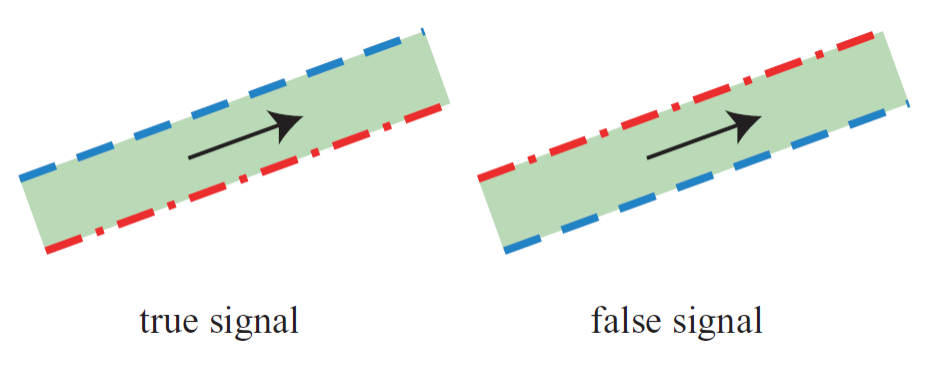
\includegraphics[width=.7\textwidth]{origami-data/wire}
    \caption{Wire gadget \cite{demaine-GFALOP-lecture}}
  \end{figure}
\end{definition}

\begin{definition}
  Our \emph{clause gadget} is the crease diagram of
  Fig. \ref{clause-creases}.
\end{definition}

\begin{figure}[h!tbp]
  \centering
  \begin{subfigure}{.3\textwidth}
    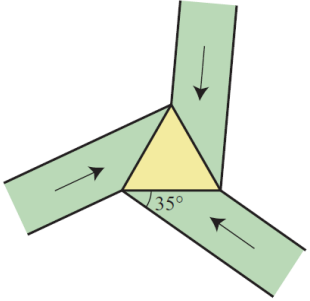
\includegraphics[width=\textwidth]{origami-data/clause}
    \caption{Crease pattern}
    \label{clause-creases}
  \end{subfigure}
  \begin{subfigure}{.3\textwidth}
    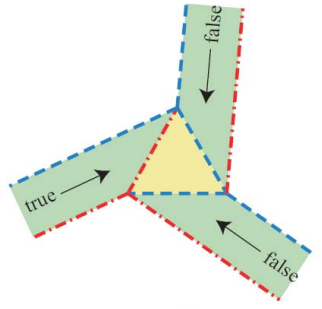
\includegraphics[width=\textwidth]{origami-data/clause-fold-1}
    \caption{Folding 1}
    \label{clause-fold-1}
  \end{subfigure}
  \begin{subfigure}{.3\textwidth}
    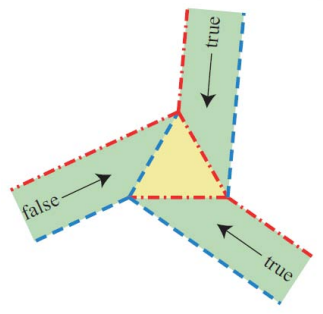
\includegraphics[width=\textwidth]{origami-data/clause-fold-2}
    \caption{Folding 2}
    \label{clause-fold-2}
  \end{subfigure}
  \caption{Clause gadget \cite{demaine-GFALOP-lecture}}
\end{figure}

\begin{lemma}
  \label{flat-clause}
  A mountain-valley assignment of the clause gadget is flat foldable
  if and only if it is a rotation of one of Figs. \ref{clause-fold-1}
  and \ref{clause-fold-2}, i.e. if and only if the three inputs are
  wires which do not all have equal value.
\end{lemma}

\begin{proof}
  We first consider the local foldability criteria at the vertices of
  the triangle. The $35^\circ$ angles are minimum at each vertex and
  hence the two creases forming then must have opposite assignment. We
  also must have either 3 mountains or 3 valleys at each vertex. These
  two constrains are illustrated by Fig. \ref{constraints-local}.
  \begin{figure}[h!tbp]
    \centering
    \begin{subfigure}{.35\textwidth}
      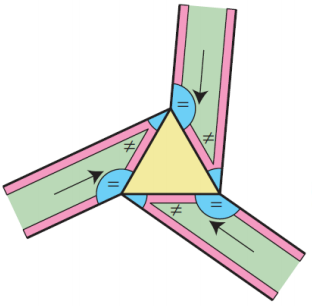
\includegraphics[width=\textwidth]{origami-data/clause-constraints}
      \caption{Vertex-local constraints}
      \label{constraints-local}
    \end{subfigure}
    \begin{subfigure}{.35\textwidth}
      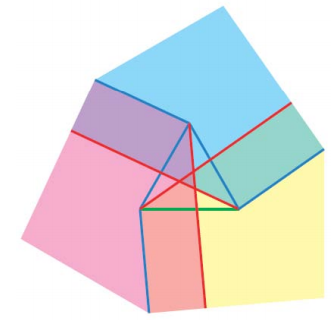
\includegraphics[width=\textwidth]{origami-data/clause-folded}
      \caption{Folded clause gadget}
      \label{clause-folded}
    \end{subfigure}
    \caption{Clause gadget folding constraints
      \cite{demaine-GFALOP-lecture}}
  \end{figure}
  This immediately implies that the parallel creases of the three
  input trapezoids must have opposite assignment, so that the three
  inputs are in fact wires. Moreover the boolean values of the wires
  determine the assignments of the creases forming the triangle. To
  finish the argument, observe that when layering is ignored, a flat
  folded clause gadget must be as depicted in Fig.
  \ref{clause-folded}. It turns out (but we omit showing this
  rigorously) that the small central triangle is an obstruction to
  flat foldability when all three wires have equal value, but
  otherwise the gadget is flat foldable.
\end{proof}

We will omit explicitly describing the split, turn, and crossover
gadgets because they're not all that interesting and can be inferred
from the final reduction, which we can now give:

\begin{proof}[Proof of \pref{flat-np}]
  By \pref{nae-hard} it suffices to give a reduction from $\NAE$ to
  $\FlatFoldability$. Suppose we are given an $\NAE$ instance $(I,T)$
  as in \pref{notallequal}. We create a crease pattern as depicted in
  Fig. \ref{flatreduction}, but with zig-zagging wires for all of our
  variables $\{x_i\}_{i \in I}$ and and analogous constructions to
  form not-all-equal clauses associated to each of the triples in
  $T$. It follows essentially from \pref{flat-clause} that this will be
  flat foldable if and only the $\NAE$ problem is satisfiable.
  \begin{figure}[h!tbp]
    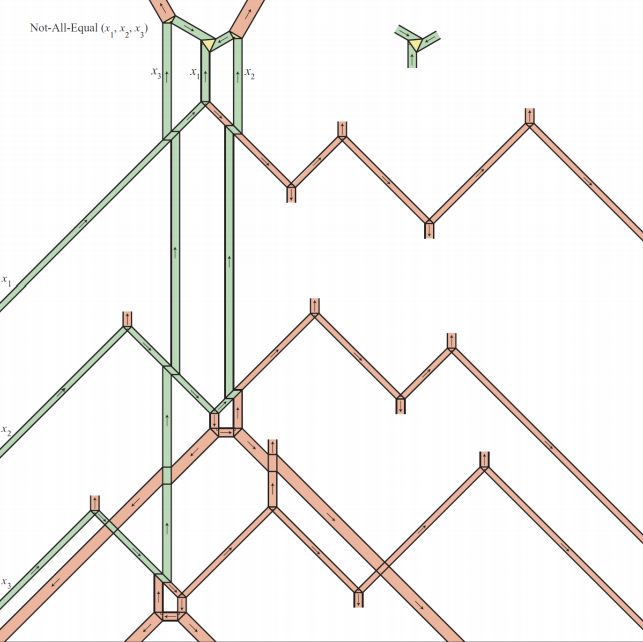
\includegraphics[width=.8\textwidth]{origami-data/flat-reduction}
    \caption{Reduction from $\NAE$ to $\FlatFoldability$
      \cite{demaine-GFALOP-lecture}}
    \label{flatreduction}
  \end{figure}
\end{proof}

%%%%%%%%%%%%%%%%%%%%%%%%%%%%%%%%%%%%%%%%%%%%%%%%%%%%%%%%%%%%%%%%%%%%%%

\section{Origami design}

We now discuss the hardness of origami design. We begin by stating the
basics of ``uniaxial bases'', which are the foundation of the ``tree
method'' of origami design, developed by R. Lang and used in real life
by him and many others.

\begin{definition}
  A \emph{uniaxial base} is a crease pattern $C$ whose faces can be
  partitioned into connected sets called flaps such that:
  \begin{enumerate}
  \item $C$ can be folded in $\R^3$ with final folded state lying
    entirely above (or in) the $x$-$y$ plane, and whose projection to
    and intersection with the $x$-$y$ plane are equal.
  \item The projection of each flap to the $x$-$y$ plane is a line
    segment, called a \emph{shadow edge}.
  \item The projection of each crease shared by distinct flaps to the
    $x$-$y$ plane is a point, called a \emph{shadow vertex}.
  \item The metric graph formed by the shadow vertices and edges is a
    tree, called the \emph{shadow tree}.
  \item Each leaf vertex of the shadow tree is the image of a unique
    point in the crease pattern.
  \end{enumerate}
\end{definition}

\begin{notation}
  If $X$ is a metric space we denote its distance function by
  $d_X$.
\end{notation}

\begin{lemma}
  \label{trivial}
  Let $C$ be a crease pattern on a finite region $P \subset \R^2$
  which is a uniaxial base with shadow tree $T$. Let $\pi \c P \to T$
  be the map given by folding $C$ and then projecting to $T$. Then
  $d_P(p,q) \ge d_T(\pi(p), \pi(q))$.
\end{lemma}

\begin{proof}
  This is fairly trivial: both folding and projecting can only
  decrease distance.
\end{proof}

The following definition describes the basic problem posed by the tree
method.

\newcommand{\UniaxialBase}{\mathsf{UniaxialBase}}

\begin{definition}
  The \emph{$\UniaxialBase$ problem} is defined as follows:
  \begin{itemize}
  \item \textsc{input}: Finite convex region $P \subset \R^2$, metric
    tree $T$.
  \item \textsc{problem}: Decide whether there is crease pattern on
    $P$ which is a uniaxial base whose shadow tree is (isomorphic to)
    $T$.
  \end{itemize}
\end{definition}

We make two reductions to deduce the hardness of $\UniaxialBase$.

\newcommand{\DiskPacking}{\mathsf{DiskPacking}}

\begin{definition}
  The \emph{$\DiskPacking$ problem} is defined as follows:
  \begin{itemize}
  \item \textsc{input}: Finite convex region $P \subset \R^2$, real
    numbers $a_1,\ldots,a_n > 0$.
  \item \textsc{problem}: Decide whether open disks $D_1,\ldots,D_n$
    of radii $a_1,\ldots,a_n$ respectively can be placed in $\R^2$
    such that their centres lie in $P$ and no two disks intersect.
  \end{itemize}
\end{definition}

\newcommand{\ThreePartition}{\mathsf{3\dash Partition}}

\begin{definition}
  The \emph{$\ThreePartition$ problem} is defined as follows:
  \begin{itemize}
  \item \textsc{input}: Positive integers $a_1,\ldots,a_{3m}$.
  \item \textsc{problem}: Decide whether we can partition
    $a_1,\ldots,a_{3m}$ into groups of $3$ with equal sum.
  \end{itemize}
\end{definition}

\begin{proposition}
  $\ThreePartition$ is $\NP$-complete.
\end{proposition}

\begin{proof}
  Omitted. See, e.g., \cite{garey-johnson}.
\end{proof}

\begin{theorem}[\cite{demaine-packing}]
  \label{packing-hard}
  $\DiskPacking$ is $\NP$-hard.
\end{theorem}

\begin{proof}
  We reduce from $\ThreePartition$.
  \begin{figure}[h!tbp]
    \centering
    \begin{subfigure}{.35\textwidth}
      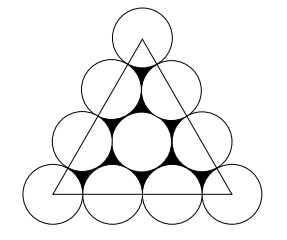
\includegraphics[width=\textwidth]{origami-data/triangle-pockets}
      \caption{Triangular region}
      \label{triangle}
    \end{subfigure}
    \begin{subfigure}{.35\textwidth}
      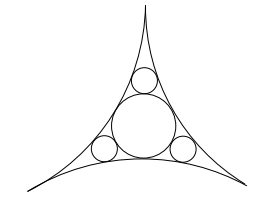
\includegraphics[width=\textwidth]{origami-data/pocket}
      \caption{Single pocket}
      \label{pocket}
    \end{subfigure}
    \caption{Reduction from $\ThreePartition$ to $\DiskPacking$}
  \end{figure}
  Suppose we are given a $\ThreePartition$ instance with input
  $a_1,\ldots,a_m$. We construct a $\DiskPacking$ instance as
  follows. Our region $P$ is an equilateral triangle. Our first input
  disks are as in Fig. \ref{triangle}, which are large enough to be
  forced into the depicted locations in any packing, except that we
  force $m$ pockets to be created. The next input disks are the
  central disks in each pocket as depicted in Fig. \ref{pocket} (again
  these placements are forced in all packings). Finally we have input
  disks $D_1,\ldots,D_m$ associated to the input $a_1,\ldots,a_m$. The
  radii of the pocket disks can be chosen---the central disk
  determined by $(\sum a_l)/m$ and the disk $D_i$ determined by
  $a_i$---such that $D_i,D_j,D_k$ can be placed in a pocket if and
  only if $a_i + a_j + a_k \le (\sum a_l)/m$, and hence the
  $\DiskPacking$ problem has a positive solution if and only if the
  original $\ThreePartition$ problem has one.
\end{proof}

\begin{corollary}
  \label{uni-hard}
  $\UniaxialBase$ is $\NP$-hard.
\end{corollary}

\begin{proof}
  Consider the tree $T$ with a central vertex $v_0$ and outer vertices
  $v_1, \ldots, v_n$ and edges $e_i = (v_0,v_i)$ of length $a_i$ for
  $1 \le i \le n$. By \pref{trivial}, any uniaxial base with shadow
  tree $T$ must contain points $p_1,\ldots,p_n$ with $d_P(p_i,p_j) \ge
  d_T(v_i,v_j) = a_i+a_j$. Thus we can place disks of radius $a_i$ at
  each $p_i$ without any intersection. This provides a reduction from
  $\DiskPacking$ to $\UniaxialBase$, so we are done by
  \pref{packing-hard}.
\end{proof}

\begin{remark}
  Our proof of \pref{uni-hard} shows that the $\NP$-hardness of
  $\UniaxialBase$ comes from the task of finding points in the crease
  pattern to lift the leaf vertices of the desired tree. In fact, this
  is where \emph{all} of the hardness lies. R. Lang's work gives an
  efficient algorithm for producing the rest of the crease pattern
  once these points are chosen.
\end{remark}

%%%%%%%%%%%%%%%%%%%%%%%%%%%%%%%%%%%%%%%%%%%%%%%%%%%%%%%%%%%%%%%%%%%%%%

\bibliographystyle{amsalpha}
\bibliography{refs}

\end{document}
